%!TEX root = qualificacao.tex
\section{AUTÔMATOS CELULARES}
\label{sec:acs}

Autômatos celulares são idealizações matemáticas simples dos sistemas naturais. Eles consistem em um reticulado de campos discretos usualmente idênticos, onde cada campo pode assumir um conjunto finitos de, geralmente, valores inteiros. Os valores dos campos evoluem em tempo discreto de acordo com regras determinísticas que especificam o valor de cada campo de acordo com os campos das vizinhanças \cite{wolfram1994cellular}.

Uma definição parecida é dada por \citeonline{weisstein2015}, que define um AC como um conjunto de células ``coloridas'' em um reticulado com forma previamente especificada que evolui ao longo de uma série de passos de tempo discreto, de acordo com um conjunto de regras baseadas nos estados de células vizinhas. As regras são aplicadas de forma iterativa para o número de passos de tempo desejado.

Os autômatos celulares são compostos por células distribuídas em um reticulado. Essas células mudam de estado ao longo de passos de tempo e de acordo com regras locais. O conjunto de células em determinado passo de tempo é denominado configuração ou estado global e são as configurações que descrevem a evolução espaço temporal de um AC. 

Autômatos celulares podem operar com reticulados em qualquer número de dimensões. Os primeiros ACs eram bidimensionais e foram criados por \citeonline{neumann1966theory} para serem usados como um modelo formal de auto reprodução de sistemas biológicos. Outro conhecido AC bidimensional é o ``Jogo da Vida'' (ou ``Game of Life''), esse AC, criado por John Conway, fez sua primeira aparição em uma coluna de jogos matemáticos \cite{GardnerM1970}. Entre os AC unidimensionais, os mais conhecidos são os do espaço elementar, que foram sistematicamente estudados por \citeonline{wolfram1983statistical}.

Independente da dimensionalidade do reticulado, é necessário definir como o AC se comportará nas bordas. Um tratamento típico é a aplicação da condição de contorno periódica nas extremidades. Ou seja, tratar reticulados unidimensionais como um anel, e bidimensionais como toro (ou toroide). Esses tratamentos podem ser visualizados na Figura \ref{fig:anel} e na Figura \ref{fig:toro}, respectivamente.  
	\begin{figure}[h!]
	  \centering
	  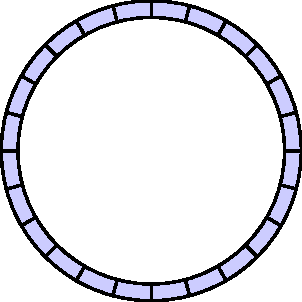
\includegraphics[width=.3\textwidth]{fig_circularList.pdf}
	  \caption{Condição de contorno periódica em um reticulado unidimensional formando um anel.}
	  \label{fig:anel}
	\end{figure}

	\begin{figure}[h!]
	  \centering
  	  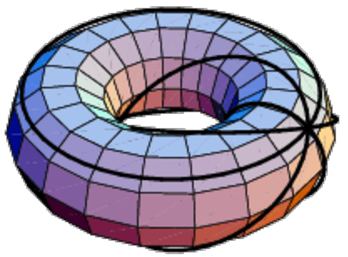
\includegraphics{fig_toro.pdf}
	  \caption{Condição de contorno periódica em um reticulado bidimensional formando um toroide.}
	  \label{fig:toro}
	\end{figure}


%Estados; regras locais; e raio
As células de um autômato celular podem apresentar $k$ estados. O valor desses estados é representado ou por cores ou por valores inteiros no intervalo $[0, k-1]$. O estado de uma célula pode ser modificado pelas funções locais, que são o conjunto de regras que determinam o novo valor de uma célula baseado em seu estado atual e nos estados das células adjacentes. Para que as funções locais atualizem os valores de uma célula, é necessário que um raio $r$ seja definido. Esse raio $r$ representa o número de células adjacentes que serão analisadas em cada direção pelas funções locais.

%vizinhanças
Além do raio, é preciso determinar o formato de vizinhança que será utilizada nos parâmetros da função local. Duas vizinhanças bem comuns em ACs bidimensionais são as vizinhanças de von Neumann \cite{weisstein2015b} e Moore \cite{weisstein2015c}. Na Figura \ref{fig:vVonNeumann} e na Figura \ref{fig:vMoore} são apresentadas, para raios de 0 a 3, as vizinhanças de von Neumann e Moore, respectivamente. No caso dos ACs unidimensionais, as vizinhanças são definidas apenas pelo raio $r$ e ele descreve quantas células a esquerda e direita da célula atual serão consideras pela função local.

	\begin{figure}[h!]
	  \centering
	  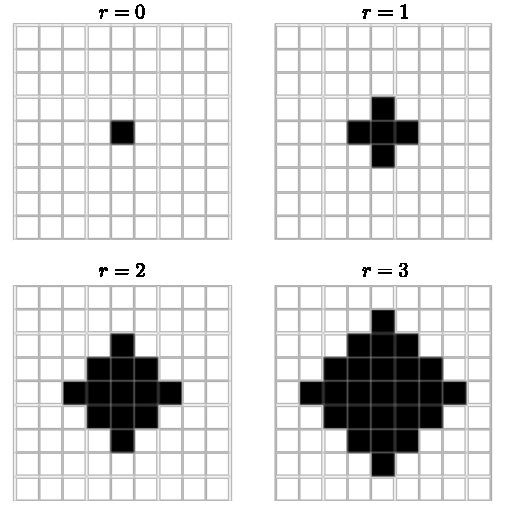
\includegraphics[width=0.45\textwidth]{fig_vVonNeumann.pdf}
	  \caption{Vizinhança de von Neumann com raio $r$ igual a 0, 1, 2 e 3. Essa foi a vizinhança utilizada nos primeiros trabalhos de von Neumann \cite{weisstein2015b}.}
	  \label{fig:vVonNeumann}
	\end{figure}

	\begin{figure}[h!]
	  \centering
  	  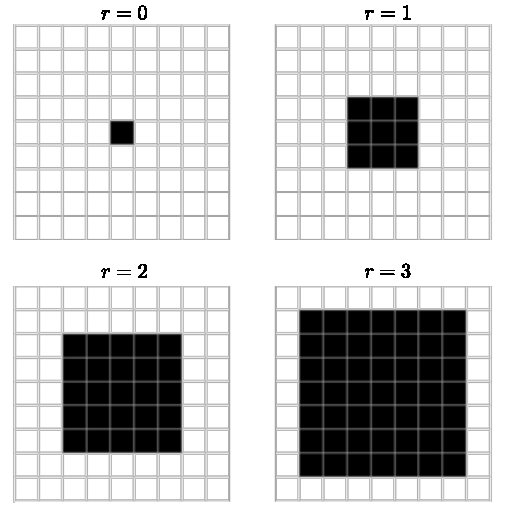
\includegraphics[width=0.45\textwidth]{fig_vMoore.pdf}
	  \caption{Vizinhança de Moore com raio $r$ igual a 0, 1, 2 e 3. Essa foi a vizinhança utilizada no jogo da vida \cite{weisstein2015c}.}
	  \label{fig:vMoore}
	\end{figure}

%Famílias de autômatos Celulares; e Autômatos Celulares Elementares.
Uma família de autômatos celulares é definida pelo raio, número de estados, tipo de vizinhança e a dimensionalidade das configurações. Autômatos celulares unidimensionais de raio $r=1$ e $k=2$ são conhecidos como a família dos autômatos celulares elementares.

Todo AC é regido por um conjunto de regras locais que determinam como ficarão as configurações no próximo passo de tempo de acordo com as configurações de vizinhança recebidas. Existem diversas maneiras de representar essas regras locais, a mais comum são as tabelas de transições. A tabela de transições é uma $n-$upla em que os elementos são todos os possíveis estados de vizinhanças de uma célula acrescentados de um estado que representa a transição que ocorrerá. A Equação \ref{eq:nupla} representa a $n$-upla da regra 30.
	\begin{equation}
	\begin{split}
	(((1,1,1),0),((1,1,0),0),((1,0,1),0),((1,0,0),1),\\
	((0,1,1),1),((0,1,0),1),((0,0,1),1),((0,0,0),0))
	\label{eq:nupla}
	\end{split}
	\end{equation}

Uma outra forma de representar uma tabela de transições é a forma icônica. Na forma icônica o bit $1$ é representado por um ícone na cor preta, e o bit $0$ por um ícone na cor branca. Cada uma das transições de estados é representada por um conjunto de ícones que representa a vizinhança na parte superior, e um ícone para representar o estado resultante após a transição na parte inferior. A Figura \ref{fig:repIconicaR30} mostra a representação icônica da regra 30.

	\begin{figure}[h!]
	  \centering
	  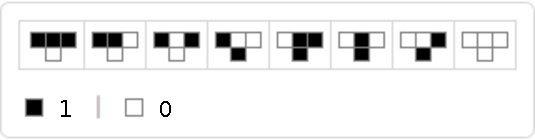
\includegraphics[width=0.6\textwidth]{fig_repIconicaR30.pdf}
	  \caption{Representação icônica da regra 30.}
	  \label{fig:repIconicaR30}
	\end{figure}

Além dessas formas de representação, ainda existe a forma $k$-aria em que, sabendo-se o valor atribuído para $k$ e $r$, elimina-se a representação das vizinhanças e deixa-se apenas as representações resultantes. Na Equação \ref{eq:karia} é possível ver a representação $k$-aria da regra 30. O número da regra é obtido ao se converter a representação $k$-aria para decimal. Esse número é um identificador único em família de autômatos celulares, ou seja, sempre representa apenas uma tabela de transições de estado.
	\begin{equation}
	(0,0,0,1,1,1,1,0)
	\label{eq:karia}
	\end{equation}

O número de regras de um espaço é definido pela Equação \ref{eq:tamFamilia}:
	\begin{equation}
	k^{k^{2r+1}}
	\label{eq:tamFamilia}
	\end{equation}

No espaço elementar há $2^{2^{3}} = 256$ regras. Aumentando o raio $r=2$, obtemos uma família de $2^{2^{5}} = 4.294.967.296$ regras. Para $k=3$ e $r=1$, obtém-se um espaço de ACs com $3^{3^{3}} = 7.625.597.484.987$ regras. Logo, é fácil perceber que qualquer modificação nas variáveis $k$ e $r$ geram famílias com número de regras muito grande. Famílias grandes de ACs representam um desafio na hora de encontrar ACs com propriedades específicas, já que procurar regras através de força bruta em um espaço muito grande se torna uma tarefa extremamente improdutiva.

Para contornar esse problema, é comum utilizar algumas propriedades estáticas para restringir as regras do espaço no qual serão feitas as buscas. Alguns exemplos de propriedades estáticas que podem auxiliar nesse ``filtro'' são o confinamento, conservabilidade de estados e conservabilidade de paridade. Todas as propriedades estáticas citadas anteriormente são detalhadas na Seção \ref{sec:propriedadesEstaticas}.

O problema da paridade é um dos problemas que envolvem fazer a ligação entre comportamento local e comportamento global de um autômato celular. Para o problema de paridade, nesse projeto, considera-se um AC binário, unidimensional e com condição de contorno periódica. Se uma configuração inicial contiver um número ímpar de estados com valor 1, o AC deve convergir para que todas as células estejam preenchidas com 1, caso contrário, ele deve convergir para todos os estados com o valor 0. Por conta da própria definição do problema, fica simples perceber que essas condições não podem ser satisfeitas em uma grelha de tamanho par, afinal uma configuração com todos os estados apresentando o mesmo valor não poderia ser um estado quiescente. Devido essa questão, pode-se dizer que as regras que solucionam o problema de paridade em ACs são \textit{perfeitas} se eles resolverem o problema de paridade em qualquer configuração inicial arbitrária para ACs de tamanho ímpar \cite{Betel2013}. Ainda em relação ao problema de paridade, Betel, De Oliveira e Flocchini (\citeyear{Betel2013}) descrevem duas propriedades básicas: se $f$ é a regra local que resolve o problema de paridade, então $f(0, \dots, 0) = 0$ e $f(1, \dots, 1) = 1$. A segunda propriedade define que para uma regra preservar a configuração de paridade ela deve apresentar número par de transições ativas. Em outras palavras, toda aplicação da regra deve levar a uma nova configuração com a mesma paridade.

Procurar uma regra que resolva o problema de paridade em autômatos celulares unidimensionais de raio 3, por exemplo, por meio de buscas por força bruta acarretaria em testar mais de 340 undecilhões de regras. Uma maneira de facilitar essa busca é restringir as regras através propriedades estáticas, mas é necessário uma forma de representar essas propriedades e até mesmo aplicar operações como intersecção e complemento entre elas. Nesse ponto que os \textit{templates} apresentam-se de uma forma interessante e útil para representar conjuntos de regras com determinada propriedade. Templates de ACs são uma generalização das tabelas de transições que permitem representar espaços inteiros de ACs \cite{Verardo2014}.